\chapter{Convolutional object detection}\label{chap3}

%##########################################
\vspace*{50 ex}

%##########################################
\paragraph*{Outline:} This chapter presents the following:
\begin{enumerate}
\setlength{\itemsep}{-0.3em}
\item Introduction
\item R-CNN
\item Fast R-CNN
\item Region proposal generation and use
\item Faster R-CNN
\item SSD
\item Comparing the methods
\end{enumerate}
\newpage

\section{Introduction}\label{chap3:intro}
In this chapter, we discuss and compare different object detection methods that utilize convolutional neural networks. In particular, we are going to look at methods that combine CNNs with region proposal classification. We further discuss, how the region proposals, also called regions of interest (ROI), are generated.

\section{R-CNN}
In 2012, Krizhevsky et al. achieved promising results with CNNs for the general image classification task, as mentioned in section 2.4.6. In 2013, Girshick et al. published a method generalizing these results to object detection. This method is called R-CNN (“CNN with region proposals”).

\subsection{General description}
R-CNN forward computation has several stages, shown in figure 3.1. First, the regions of interest are generated. The RoIs are category-independent bounding boxes that have a high likelihood of containing an interesting object. In the paper, a separate method called Selective Search, is used for generating these, but other region generation methods can be used instead. Selective Search, along with other region proposal generation techniques, is discussed in further detail in section 3.3.

Next, a convolutional network is used to extract features from each region proposal. The sub-image contained in the bounding-box is warped to match the input size of the CNN and then fed to the network. After the network has extracted features from the input, the features are input to support vector machines (SVM) that provide the final classification.
\noindent
\begin{figure}
	\centering
	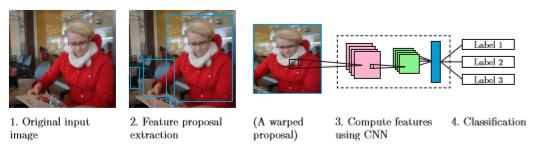
\includegraphics[width=1\linewidth]{img5} 
	\caption{ Stages of R-CNN forward computation.}\href{https://www.semanticscholar.org/paper/Object-detection-from-images-using-convolutional-Stenroos/a6ee78ea9c68d99d6545227fed925a721337bb16/figure/4}{link}
	\label{fig:img5}
\end{figure}
\noindent
The method is trained in multiple stages, beginning with the convolutional network. After the CNN has been trained, the SVMs are fitted to the CNN features. Finally, the region proposal generating method is trained.

\subsection{Drawbacks}
R-CNN is an important method, because it provided the first practical solution for object detection using CNNs. Being the first, it has many drawbacks that have been improved upon by later methods.

In his 2015 paper for Fast R-CNN, Girshick lists three main problems of R-CNN:

First, training consists of multiple stages, as described above. Second, training is expensive. For both SVM and region proposal training, features are extracted from each region proposal and stored on disk. This requires days of computation and hundreds of gigabytes of storage space. Third, and perhaps most important, object detection is slow, requiring almost a minute for each image, even on a GPU. This is because the CNN forward computation is performed separately for every object proposal, even if the proposals originate from the same image or overlap each other.


\section{Fast R-CNN}
Fast R-CNN published in 2015 by Girshick provides a more practical method for object recognition. The main idea is to perform the forward pass of the CNN for the entire image, instead of performing it separately for each ROI.

\subsection{General description}

The general structure of Fast R-CNN is illustrated in figure 3.2. The method receives as input an image plus regions of interest computed from the image. As in R-CNN, the RoIs are generated using an external method. The image is processed using a CNN that includes several convolutional and max pooling layers. The convolutional feature map that is generated after these layers is input to a RoI pooling layer. 

This extracts a fixed-length feature vector for each RoI from the feature map. The feature vectors are then input to fullyconnected layers that are connected to two output layers: a softmax layer that produces probability estimates for the object classes and a real-valued layer that outputs bounding box co-ordinates computed using regression (meaning refinements to the initial candidate boxes).

\begin{figure}
	\centering
	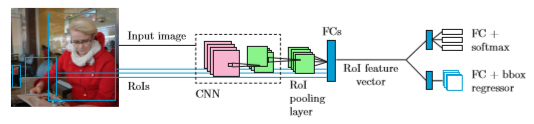
\includegraphics[width=0.9\linewidth]{img6}
	\caption{Stages of Fast R-CNN forward computation.} \href{https://www.semanticscholar.org/paper/Object-detection-from-images-using-convolutional-Stenroos/a6ee78ea9c68d99d6545227fed925a721337bb16/figure/5}{link}
	\label{fig:img6}
\end{figure}

\subsection{Classification performance}
According to the authors, Fast R-CNN provides significantly shorter classification time compared to regular R-CNN, taking less than a second on a state-of-the-art GPU. This is mainly due to using the same feature map for each RoI.

As the detection time decreases, the overall computation time begins to depend significantly on the performance of the region proposal generation method. The RoI generation can thus form a computational bottleneck. Additionally, when there are many RoIs, the time spent on evaluating the fully-connected layers can dominate the evaluation time of the convolutional layers. Classification time can be accelerated by approximately 30\% if the fully-connected layers are compressed using truncated singular value decomposition. This results in a slight decrease in precision, however.

\subsection{Training}
According to the original publication, Fast R-CNN is more efficient to train than R-CNN, with nine-fold reduction in training time. The entire network (including the RoI pooling layer and the fully-connected layers) can be trained using the back-propagation algorithm and stochastic gradient descent. Typically, a pre-trained network is used as a starting point and then fine-tuned. Training is done in mini-batches of N images. R/N RoIs are sampled from each mini-batch image. The RoI samples are assigned to a class, if their intersection over union with a ground-truth box is over 0.5. Other RoIs belong to the background class.

As in classification, RoIs from the same image share computation and memory usage. For data augmentation, the original image is flipped horizontally with probability 0.5. The softmax classifier and the bounding box regressors are fine-tuned together using a multi-task loss function, which considers both the true class of the sampled RoI and the offset of the sampled bounding box from the true bounding box.

\section{Region proposal generation and use}
To use R-CNN and Fast R-CNN, we need a method for generating the classagnostic regions of interest. Next, we are going to discuss general principles of RoI generation, and have a closer look at two popular methods: Selective Search and Edge Boxes.

\subsection{Overview}
The aim of region proposal generation in object detection is to maximize recall i.e. to generate enough regions so that all true objects are recovered. The generator is less concerned with precision, since it is the task of the object detector to identify correct regions from the output of the region proposal generator.

However, the amount of proposals generated affects performance. As mentioned in section 2.3.2, there are two main approaches to region generation: dense set generation and sparse set generation.

Dense set solutions attempt to generate by brute force an exhaustive set of bounding boxes that includes every potential object location. This can be achieved by sliding a detection window across the image. However, searching through every location of the image is computationally costly and requires a fast object detector. Additionally, different window shapes and sizes need to be considered. Thus, most sliding window methods limit the amount of candidate objects by using a coarse step-size and a limited number of fixed aspect ratios.

Most region proposals in a dense set do not contain interesting objects. These proposals need to be discarded after the object detection phase. Detection results can be discarded, if they fall behind a predefined confidence threshold or if their confidence value is below a local maximum (non-maximum suppression).

Instead of discarding the regions after the object detection stage, the region proposal generator itself can rank the regions in a class-agnostic way and discard low-ranking regions. This generates a sparse set of object detections. Similarly to dense set methods, thresholding and non-maximum suppression can be implemented after the detection phase to further improve the detection quality. Sparse set solutions can be grouped into unsupervised and supervised methods.

One of the most popular unsupervised methods is Selective Search (see section 3.3.2), which utilizes an iterative merging of superpixels. There are also other methods that use the same approach. Another approach is to rank the objectness of a sliding window. A popular example of this is Edge Boxes (see section 3.3.3), which calculates the objectness score by calculating the number of edges within a bounding box and by subtracting the number of edges that overlap the box boundary. There is also a third group of methods based on seed segmentation.

Supervised methods treat region proposal generation as a classification or a regression problem. This means using a machine learning algorithm, such as a support vector machine. It is also possible to use a convolutional network to generate the regions of interest. An example of using a CNN for calculating the bounding boxes is Multi-Box.

Certain advanced object detection methods, such as Faster R-CNN described in 3.4.1, use parts of the same convolutional network both for generating the region proposals and for detection. We call these kinds of methods integrated methods.

\subsection{Selective Search}
Selective Search utilizes a hierarchical partitioning of an image to create a sparse set of object locations. The main design philosophy is not to use a single strategy, but to combine the best features of bottom-up segmentation and exhaustive search. The authors had three main design considerations: the search should capture all scales, be diverse i.e. not use any single strategy for grouping regions and be fast to compute.

The algorithm begins by creating a set of small initial regions using a method called Graph Based Image Segmentation designed by Felzenszwalb and Huttenlocher. The method creates a set of regions called superpixels. The superpixels are internally nearly uniform. Combined, they span the entire image, but individually they should not span different objects. 

Selective Search then continues by iteratively grouping the regions together using a greedy algorithm, beginning with the two most similar regions. Many complimentary measures are used to compute the similarity. These measures consider colour similarity (by computing a colour histogram), texture similarity (by computing a SIFT-like measure), size of the regions (small regions should be merged earlier) and how well the regions fit together (gaps should be avoided). The grouping phase ends when every region has been combined.

The hypothetical object locations thus generated are then ordered by the likelihood of the location containing an object. In practice, the locations are ordered based on the order in which they were grouped together by the different measures. A certain element of randomness is added to prevent large objects from being favoured too much. Lower-ranking duplicates are removed. 

Both the region generating method and the similarity measures were selected to be fast to compute, making the method fast in general. In addition to using diverse similarity measures, the search can be further diversified by using complementary colour spaces (to ensure lighting invariance) and using complementary starting regions.

\subsection{Edge Boxes}
As the name suggests, Edge Boxes is based on detecting objects from edge maps. The main contribution of the authors of the method is the observation that the number of edge contours wholly enclosed by a bounding box is correlated with the likelihood that the box contains an object.

First, the edge map is calculated using a method by the same authors called Structured Edge Detector. Then, thick edge lines are thinned using non-maximum suppression. Instead of operating on the edge pixels directly, the pixels are grouped using a greedy algorithm. An affinity measure is devised to calculate whether edge groups are part of the same contour.

The region proposals are found by scanning the image using the traditional sliding window method and calculating an objectness score at each position, aspect ratio and scale. The score is calculated by summing the edge strength of edge groups that lie completely within the box and subtracting the strength of edge groups that are part of a contour that cross the box boundary. Promising regions are then further refined.


\section{Faster R-CNN}
In the experimental section of this thesis, we will focus mostly on Faster R-CNN. There are, however, several state-of-the-art algorithms with an improved computation time or accuracy. Next, we will describe two of these algorithms first faster R-CNN in this section and SSD (see section 3.6) in next section.

\subsection{Overview}
Faster R-CNN by Ren et al. is an integrated method. The main idea is to use shared convolutional layers for region proposal generation and for detection. The authors discovered that feature maps generated by object detection networks can also be used to generate the region proposals. The fully convolutional part of the Faster R-CNN network that generates the feature proposals is called a region proposal network (RPN). The authors used Fast R-CNN architecture for the detection network.

A Faster R-CNN network is trained by alternating between training for RoI generation and detection. First, two separate networks are trained. Then, these networks are combined and fine-tuned. During fine-tuning, certain layers are kept fixed and certain layers are trained in turn.

The trained network receives a single image as input. The shared fully convolutional layers generate feature maps from the image. These feature maps are fed to the RPN. The RPN outputs region proposals, which are input, together with the said feature maps, to the final detection layers. These layers include a RoI pooling layer and output the final classifications.

Using shared convolutional layers, region proposals are computationally almost cost-free. Computing the region proposals on a CNN has the added benefit of being realizable on a GPU. Traditional RoI generation methods, such as Selective Search, are implemented using a CPU.

For dealing with different shapes and sizes of the detection window, the method uses special anchor boxes instead of using a pyramid of scaled images or a pyramid of different filter sizes. The anchor boxes function as reference points to different region proposals centred on the same pixel.


\subsection{General description}
In this section, we briefy introduce the key aspects of the Faster R-CNN. We refer readers to the original paper (\cite{NIPS2015_5638}) for more technical details.

In the RPN, the convolution layers of a pre-trained network are followed by a 3 $\times$ 3 convolutional layer. This corresponds to mapping a large spatial window or receptive field (e.g., 228 $\times$ 228 for VGG16) in the input image to a low-dimensional feature vector at a center stride (e.g., 16 for VGG16). Two 1 $\times$ 1 convolutional layers are then added for classification and regression branches of all spatial windows.

To deal with different scales and aspect ratios of objects, anchors are introduced in the RPN. An anchor is at each sliding location of the convolutional maps and thus at the center of each spatial window. Each anchor is associated with a scale and an aspect ratio. Following the default setting of, we use 3 scales (1282, 2562, and 5122 pixels) and 3 aspect ratios (1: 1, 1: 2, and 2: 1), leading to k = 9 anchors at each location. Each proposal is parameterized relative to an anchor. Therefore, for a convolutional feature map of size W $\times$H, we have at most W H k possible proposals. We note that the same features of each sliding location are used to regress k=9 proposals, instead of extracting k sets of features and training a single regressor.t Training of the RPN can be done in an end-to-end manner using stochastic gradient descent (SGD) for both classification and regression branches. For the entire system, we have to take care of both the RPN and Fast R-CNN modules since they share convolutional layers. In this paper, we adopt the approximate joint learning strategy proposed in (\cite{NIPS2015_5638}). The RPN and Fast R-CNN are trained end-to-end as they are independent. Note that the input of the Fast R-CNN is actually dependent on the output of the RPN. For the exact joint training, the SGD solver should also consider the derivatives of the RoI pooling layer in the Fast R-CNN with respect to the coordinates of the proposals predicted by the RPN. However, as pointed out by (\cite{NIPS2015_5638}), it is not a trivial optimization problem.

\section{ SSD}
In the experimental section of this thesis, we will focus mostly on Faster R-CNN. There are, however, several state-of-the-art algorithms with an improved computation time or accuracy. Next, we will describe SSD in this section and faster R-CNN (see section 3.5) described in previous section.


\subsection{Overview}
The Single Shot MultiBox Detector(SSD) takes integrated detection even further. The method does not generate proposals at all, nor does it involve any resampling of image segments. It generates object detections using a single pass of a convolutional network.

Somewhat resembling a sliding window method, the algorithm begins with a default set of bounding boxes. These include different aspect ratios and scales. The object predictions calculated for these boxes include offset parameters, which predict how much the correct bounding box surrounding the object differs from the default box.

The algorithm deals with different scales by using feature maps from many different convolutional layers (i.e. larger and smaller feature maps) as input to the classifier. Since the method generates a dense set of bounding boxes, the classifier is followed by a non-maximum suppression stage that eliminates most boxes below a certain confidence threshold.


\begin{figure}
	\centering
	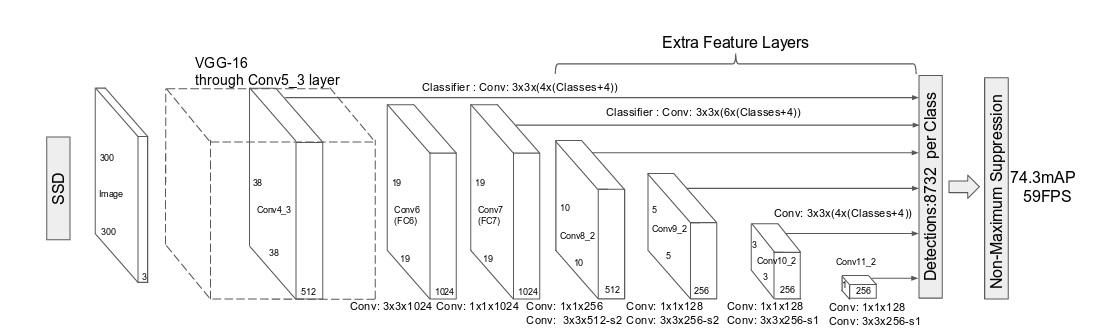
\includegraphics[width=1.0\linewidth]{img17}
	\caption{SSD Architecture} \href{https://towardsdatascience.com/learning-note-single-shot-multibox-detector-with-pytorch-part-1-38185e84bd79}{link}
	\label{fig:img17}
\end{figure}


\section{Comparing the methods}
Above, we described how Fast R-CNN is faster and more accurate than regular R-CNN. But how does Fast R-CNN perform compared to the above mentioned advanced methods?

Liu et al. [36] compared the performance of Fast R-CNN, Faster R-CNN and SSD on the PASCAL VOC 2007 test set (see section 4.5 for discussion of the standard benchmarks). When using networks trained on the PASCAL VOC 2007 training data, Fast R-CNN achieved a mean average precision (mAP) of 66.9. Faster R-CNN performed slightly better, with a mAP of 69.9. SSD achieved a mAP of 68.0 with input size 300 x 300 and 71.6 with input size 512 x 512. As the standard implementations of Fast R-CNN and Faster R-CNN use 600 as the length of the shorter dimension of the input image, SSD seems to perform better with similarly sized images. However, SSD requires extensive use of data augmentation to achieve this result. Fast R-CNN and Faster RCNN only use horizontal flipping, and it is currently unknown, whether they would benefit from additional augmentation.

While the advanced methods are more precise than Fast R-CNN, the real improvements come from speed. When most of the detections with a low probability are eliminated using thresholding and non-maximum suppression, SSD512 can run at 19 FPS on a Titan X GPU. Meanwhile, Faster R-CNN with a VGG-16 architecture performs at 7 FPS. The original authors of Faster R-CNN report a running time of 5 FPS i.e. 0.2 s per image. Fast R-CNN has approximately the same evaluation speed, but requires additional time for calculating the region proposals. Region generation time depends on the method, with Selective Search requiring 2 seconds per image on a CPU and Edge Boxes requiring 0.2 seconds per image.

%\section{Summary}
%In this chapter...